\chapter{Implementación y experimentación}\label{chapter:implementation}
En el presente capítulo se presentan los elementos prácticos que han sido empleados para 
materializar la solución conceptualizada en el diseño previo. El objetivo principal es 
detallar cómo se implementaron las diversas tecnologías, metodologías y herramientas 
seleccionadas para construir un sistema funcional que cumpla con los 
requisitos establecidos y los objetivos trazados.

Se expondrá en primer lugar la identidad del sitio web, destacando las decisiones relacionadas 
con su diseño visual y los elementos que refuerzan su alineación con los valores de marca del 
Jardín Botánico Nacional de Cuba. Posteriormente, se describirán de manera estructurada los 
procesos técnicos y las decisiones tomadas durante la implementación, haciendo énfasis en 
aspectos clave como la selección de tecnologías, la organización del código y las estrategias 
empleadas para integrar y probar los componentes del sistema.

Además, se discutirán los retos encontrados durante esta etapa y las soluciones 
adoptadas para superarlos, asegurando que el producto final sea técnicamente robusto 
y alineado con las necesidades del proyecto.

Se explicarán por separado las soluciones propuestas para las dos problemáticas 
abordadas en el capítulo anterior. Este enfoque se adopta porque cada problemática puede 
considerarse un problema independiente, lo que facilita una comprensión más clara y detallada 
de la solución final.

Adicionalmente, se incluyen las primeras pruebas experimentales realizadas con la solución implementada, 
con el fin de evaluar su desempeño y validar que los resultados obtenidos cumplen con las 
expectativas definidas en las fases iniciales. Estos experimentos no solo verifican el cumplimiento 
funcional, sino que también permiten identificar posibles áreas de mejora o ajuste, 
garantizando que el sistema sea escalable y adaptable a futuros requerimientos.



\section{Identidad del sitio}
El sistema desarrollado como resultado de este trabajo ha sido nombrado\newline \textbf{BotaniQ}, un nombre 
que refleja de manera directa su propósito y esencia. La elección de este nombre surge de la 
combinación de dos elementos clave: la palabra \textit{``botánica''}, que alude al estudio de las plantas, 
y la letra \textit{``Q''}, que hace referencia a \textit{``query''} (significa consulta en inglés),
resaltando su función principal como una herramienta para la consulta y gestión de información sobre plantas medicinales. 
Este nombre busca transmitir simplicidad, profesionalismo y un enfoque claro en la temática del 
proyecto, a la vez que facilita su identificación y asociación con su objetivo principal.
En la Figura \ref{fig:botaniq} se muestra el logotipo de BotaniQ.

\begin{figure}[ht!]
    \centering
    
\includegraphics[width=0.25\textwidth]{Images/botaniq.png}
    \caption{Logotipo de BotaniQ}
    \label{fig:botaniq}
\end{figure}

Las interfaces de BotaniQ están diseñadas para reflejar y reforzar un valor de marca que pueda 
asociarse directamente con el Jardín Botánico Nacional de Cuba. Para lograr este propósito, 
se ha adoptado una paleta cromática basada en los colores primario y secundario presentes en 
el logotipo de dicha institución, asegurando así una identidad visual coherente y representativa.
La paleta de colores se muestra en la Figura \ref{fig:palette}.

\begin{figure}[ht!]
    \centering
    
\includegraphics[width=1\textwidth]{Images/palette.png}
    \caption{Paleta de colores}
    \label{fig:palette}
\end{figure}

Para garantizar que el diseño del sitio web BotaniQ transmita una identidad visual acorde a su 
propósito, se seleccionaron fuentes tipográficas que equilibran profesionalismo, claridad y frescura, 
alineadas con la temática botánica y científica del proyecto. Estos estilos son accesibles
libre de costo desde el sitio: \href{https://fonts.google.com/}{Google Fonts}. 
Una muestra de estos estilos se puede apreciar en la Figura \ref{fig:fonts}.

\begin{itemize}
    \item Estilo primario: \texttt{Montserrat Alternates}
    \item Estilo secundario: \texttt{Quicksand}
    \item Estilo complementario: \texttt{Sniglet}
\end{itemize}


\begin{figure}[ht!]
    \centering
    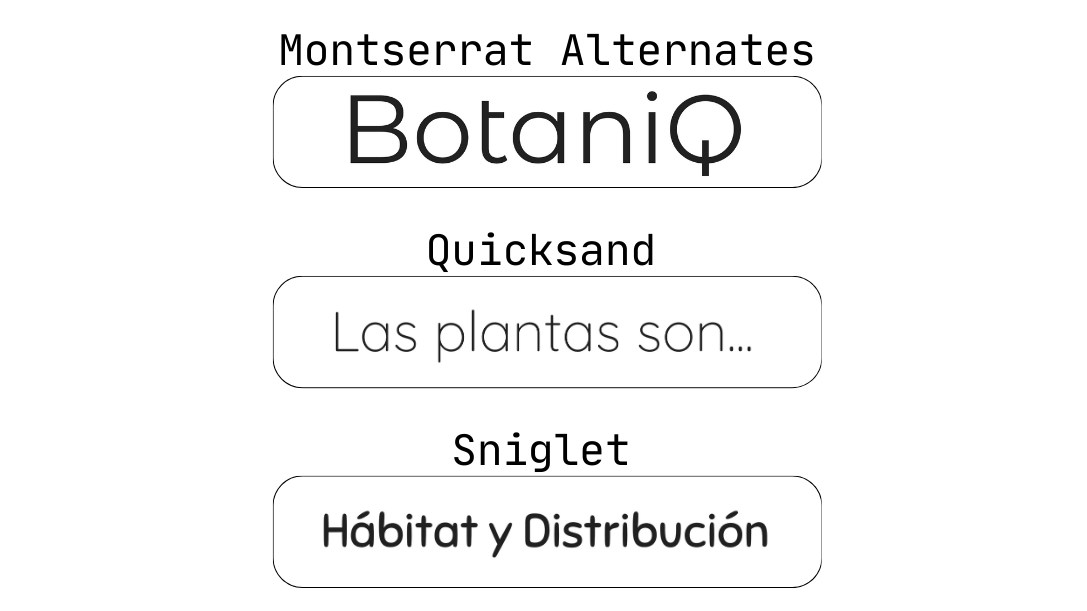
\includegraphics[width=1\textwidth]{Images/fonts.png}
    \caption{Fuentes tipográficas}
    \label{fig:fonts}
\end{figure}



\section{Solución al problema de Extracción de información}
Para implementar esta solución, se seleccionó 
\textbf{Python}\footnote{Visitar en \url{https://www.python.org}} como lenguaje de programación 
debido a su versatilidad, facilidad de uso y la sólida comunidad que lo respalda, ofreciendo 
una amplia variedad de bibliotecas para diversas tareas. Python es un lenguaje de 
programación interpretado, de alto nivel y multiparadigma, que permite trabajar con estilos 
como la programación orientada a objetos, funcional y procedimental. Su diseño enfatiza la 
legibilidad del código, lo que facilita el desarrollo y mantenimiento de proyectos.

En este contexto, se eligieron las bibliotecas 
\texttt{PyMuPDF}\footnote{Visitar en \url{https://pypi.org/project/PyMuPDF/}} y 
\texttt{pdfplumber}\footnote{Visitar en \url{https://pypi.org/project/pdfplumber/}} para 
abordar la lectura de los documentos en formato \textit{PDF}. La biblioteca \texttt{PyMuPDF} 
fue escogida principalmente por su extensa documentación y su eficacia en la extracción de 
texto de manera uniforme, lo que resulta fundamental para garantizar una base inicial 
consistente de los datos extraídos. Por otro lado, \texttt{pdfplumber} se seleccionó por las 
ventajas que ofrece en términos de manejo del diseño del documento, particularmente su 
capacidad para identificar y encuadrar bloques de texto.

La información extraída será almacenada en un archivo en formato \textit{JSON}. Este formato 
es ampliamente utilizado en la actualidad debido a su capacidad para representar datos de 
manera estructurada y su gran adaptabilidad en los sistemas computacionales modernos. 
\textit{JSON} es un formato ligero y de fácil lectura tanto para humanos como para máquinas, 
lo que lo convierte en una opción ideal para la interoperabilidad entre diferentes sistemas 
y plataformas, especialmente en aplicaciones web y servicios API.

Tal como se expuso en el capítulo anterior, se adoptará un enfoque basado en \textit{template filling} 
para estructurar la información extraída. Las plantillas se implementarán como diccionarios de Python, 
una estructura de datos que permite almacenar información en pares clave-valor de forma eficiente. 
Los diccionarios son fundamentales para garantizar una representación coherente y ordenada de los datos, 
facilitando su posterior transformación al formato \textit{JSON}.

Para la implementación del flujo de llenado de plantillas, se adoptó un estilo de programación imperativa. 
El llenado de las plantillas 
se realizó de manera jerárquica, progresando desde los niveles más generales hacia los más específicos. 
En otras palabras, primero se completaron los atributos simples de la plantilla principal, y posteriormente 
se procedió al llenado de los atributos que corresponden a subplantillas.

Este enfoque permite encapsular las reglas de llenado de las subplantillas en algoritmos independientes, 
lo que no solo mejora la modularidad del código, sino que también facilita la comprensión y el mantenimiento 
del flujo de trabajo. Al trabajar con subplantillas de manera autónoma, se asegura que cada componente de la 
plantilla sea manejado de forma eficiente y aislada, reduciendo la complejidad del sistema general y permitiendo 
futuros ajustes o ampliaciones de manera más sencilla.

Durante el desarrollo del algoritmo para la extracción de las monografías, surgieron ciertos problemas que 
requirieron ser resueltos sobre la marcha. Estas dificultades se debieron, en algunos casos, a excepciones 
en las reglas de llenado previamente definidas, ya sea por errores tipográficos en el texto original o por 
inconsistencias durante el proceso de extracción del contenido del libro. Entre los problemas identificados 
se encuentran los siguientes:

\begin{itemize}
    \item Secciones en las que no se detectó la palabra clave que determina su inicio fueron insertadas 
    erróneamente como una continuación de la sección previamente identificada.
    \item Duplicación de nombres de monografías idénticos, lo que generaba conflictos al intentar 
    utilizarlos como claves en los atributos de la plantilla.
    \item Inclusión de pies de página de las imágenes dentro del texto extraído.
    \item Inclusión de números de página entre el texto.
    \item Fragmentación de palabras en el texto debido al uso de guiones (\texttt{-}) cuando estas no 
    cabían en la línea del texto original, lo que afectaba la integridad del texto plano extraído.
\end{itemize}

La solución a estos problemas no fue particularmente compleja de identificar. Algunos casos, debido a su 
naturaleza limitada y a la falta de un patrón recurrente en el texto, fueron resueltos de forma directa 
y específica mediante soluciones personalizadas adaptadas a cada caso puntual.

Al finalizar el algoritmo de extracción, cada atributo que almacena una cadena de texto queda representado 
en un formato plano. Esto significa que no se preservan las separaciones de párrafos, siendo el contenido 
una simple secuencia de oraciones concatenadas. Además, en ocasiones donde el texto original contiene 
listas de elementos, estas se presentan como elementos continuos separados únicamente por espacios. 
Este tipo de formato puede dificultar la lectura y la interpretación del contenido, lo que hace 
necesario estructurarlo de manera más clara para mejorar su comprensión. Incluso una medida sencilla, 
como la inclusión de saltos de línea (\verb|\n|), puede contribuir significativamente a mejorar la legibilidad.

Para abordar este problema, se aprovecha el poder de los modelos de lenguaje para interpretar y 
generar texto de manera coherente. En este caso, se utilizó el modelo \texttt{gemini-1.5-flash} de
\textbf{Gemini}\footnote{Visitar a través de Google AI Studio en \url{https://aistudio.google.com/}}, desarrollado por Google, 
cuya elección se fundamenta en la disponibilidad de una API gratuita y su integración sencilla con lenguajes 
como Python para tareas automatizadas. Este modelo ha demostrado excelentes resultados en procesos de 
procesamiento y generación de texto. Para garantizar que el texto resultante cumpla con los requisitos esperados, 
se aplicaron técnicas de ingeniería de prompts diseñadas para guiar al modelo hacia la generación de resultados 
precisos y adecuados.

El resultado final es una plantilla completa, organizada y bien estructurada, con datos listos para ser leídos 
e interpretados de manera eficiente. Esta transformación mejora la presentación visual del contenido  
y optimiza su utilidad en contextos prácticos.

A continuación, se procedió a extraer la información correspondiente a la agrupación de plantas según sus aplicaciones. 
Similar al caso anterior, se presentaron algunos inconvenientes debido a inconsistencias en las reglas definidas 
durante el diseño de la solución o a limitaciones inherentes a la biblioteca utilizada para la extracción de texto. 
Entre los problemas identificados se encuentran:
 
\begin{itemize}
    \item En ciertos casos puntuales, nombres de plantas que continúan en la siguiente línea no fueron 
    detectados correctamente. Esto ocurrió porque, al no estar separados por un guion (\texttt{-}), 
    no se considera un corte de palabra, y la palabra en la línea siguiente comienza con mayúscula, 
    lo que impide la asociación automática.
    \item En un caso específico, un nombre de aplicación no fue identificado en su posición correspondiente, 
    lo que resultó en que su contenido fuera erróneamente incluido dentro de la aplicación anterior.
\end{itemize}

Dado que estos problemas son casos excepcionales y no recurrentes, se abordaron mediante correcciones 
directas en el código implementado.

El resultado final es una plantilla estructurada y completamente llena, representada en formato \textit{JSON}, 
que está lista para ser utilizada en otros entornos computacionales. 




\section{Solución al problema del Sistema de gestión y visualización: BotaniQ}
En el desarrollo de BotaniQ, se emplearon tecnologías modernas y ampliamente utilizadas en la industria 
para garantizar un sistema robusto, eficiente y escalable. Estas herramientas fueron seleccionadas 
cuidadosamente para abordar los requerimientos específicos del proyecto, permitiendo una implementación 
organizada y una experiencia de usuario óptima.

Para el frontend, se utilizó 
\textbf{React} \footnote{Visitar en \url{https://react.dev}}
en combinación con 
\textbf{TypeScript}\footnote{Visitar en \url{https://www.typescriptlang.org}}. 
React es una biblioteca de JavaScript enfocada en la creación de interfaces de usuario dinámicas y reactivas, estructuradas en componentes 
modulares que facilitan el desarrollo y la reutilización de elementos visuales. TypeScript, al ser un 
superconjunto tipado de JavaScript, aporta seguridad al proceso de desarrollo, permitiendo detectar 
errores antes de la ejecución y promoviendo un código más estructurado, lo cual es esencial en un 
proyecto de esta magnitud. Esta combinación mejora la experiencia del usuario final con una 
interfaz intuitiva, y facilita el mantenimiento y la escalabilidad del sistema.

En el backend, se optó por 
\textbf{ASP.NET Core}\footnote{Visitar en \url{https://dotnet.microsoft.com/en-us/apps/aspnet}}
como marco de desarrollo, una plataforma de código abierto diseñada para construir aplicaciones modernas 
de alto rendimiento. Este framework permite desarrollar servicios web estructurados que manejan eficientemente la lógica 
del negocio y el acceso a datos. 
La implementación del backend se organizó en capas previamente definidas: la capa de datos, la capa de acceso a datos y 
la capa de servicios, cada una desarrollada como una biblioteca dinámica (DLL) utilizando
\textbf{C\#}\footnote{Visitar en \url{https://dotnet.microsoft.com/en-us/languages/csharp}}.

La información se gestiona mediante una base de datos 
\textbf{PostgreSQL}\footnote{Visitar en \url{https://www.postgresql.org}},
un sistema de gestión de bases de datos relacional reconocido por su rendimiento y capacidad para manejar datos 
estructurados. A pesar de su naturaleza relacional, PostgreSQL ofrece características similares a las bases de datos NoSQL, 
como la capacidad de almacenar datos en formato JSON. Esta flexibilidad nos permite almacenar las monografías de plantas de 
manera eficiente, asegurando que, a pesar de que algunas secciones puedan estar vacías, todas las monografías sigan el mismo 
esquema gracias a la técnica de template filling. El backend es responsable de procesar las solicitudes, interactuar con 
PostgreSQL a través de la capa de acceso a datos y exponer los datos mediante servicios web que pueden ser consumidos por el frontend.

Estas tecnologías trabajan de forma integrada para garantizar 
un flujo de datos coherente y confiable entre el cliente y el servidor, asegurando que los usuarios de 
BotaniQ puedan acceder a la información de manera rápida y eficiente. Estas herramientas modernas y 
probadas en entornos de producción aseguran que el sistema sea robusto, mantenible y esté preparado para 
futuros requerimientos.

Esta estructura tecnológica se ilustra en la Figura \ref{fig:techs}, proporcionando una visión 
clara de cómo se integran los diferentes componentes del sistema.

\begin{figure}[ht!]
    \centering
    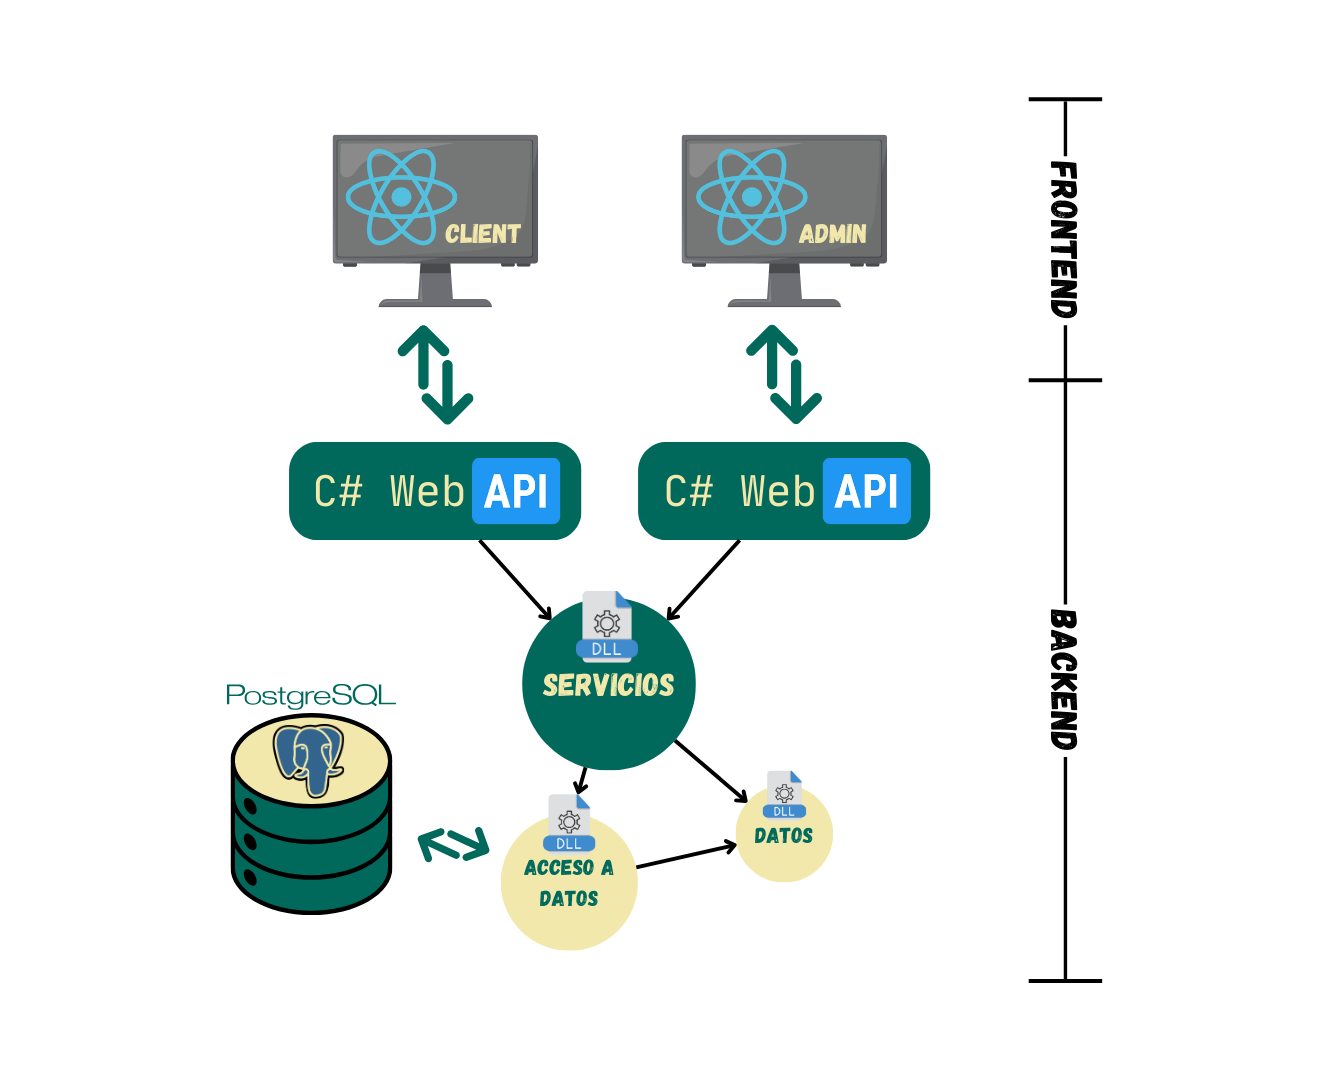
\includegraphics[width=0.9\textwidth]{Images/techs.png}
    \caption{Estructura tecnológica del sistema}
    \label{fig:techs}
\end{figure}

En ambos proyectos de frontend de BotaniQ, el desarrollo se realizó siguiendo el diseño de identidad del sitio, 
que se basa en ofrecer una experiencia visual coherente y profesional que refleje la marca asociada al 
Jardín Botánico Nacional de Cuba. A lo largo del proceso de implementación, se prestó especial atención a la 
adaptabilidad de la interfaz, asegurando que el sitio fuera completamente responsivo y brindara una experiencia 
de usuario óptima en diversos dispositivos, desde computadoras de escritorio hasta teléfonos móviles y tabletas.

Para lograr esta adaptabilidad, se utilizó 
\textbf{Tailwind CSS}\footnote{Visitar en \url{https://tailwindcss.com}},
un framework de CSS altamente flexible y eficiente que permite una personalización precisa y una creación de 
interfaces de usuario rápida y efectiva. Con Tailwind, fue posible aplicar un enfoque de diseño móvil primero, 
garantizando que la interfaz respondiera de manera eficiente a las diferentes resoluciones de pantalla sin 
perder la coherencia en su estructura visual. Además, el uso de clases utilitarias de Tailwind facilitó el 
diseño modular, lo que mejoró la mantenibilidad y escalabilidad del sistema.

Adicionalmente, se implementó 
\textbf{Flowbite}\footnote{Visitar en \url{https://flowbite.com}},
una biblioteca de componentes basada en Tailwind CSS, para acelerar el desarrollo y asegurar una interfaz de 
usuario consistente. Flowbite proporcionó una serie de componentes preconstruidos y personalizables, como 
botones, formularios y modales, lo que permitió integrar elementos interactivos con facilidad y sin necesidad 
de construir cada componente desde cero. Gracias a la combinación de Tailwind y Flowbite, se logró una 
interfaz visualmente atractiva, funcional y alineada con los principios de diseño del sitio.

Por otro lado, en el desarrollo del backend de BotaniQ, se implementaron las APIs necesarias para exponer 
los servicios que permiten la interacción entre el frontend y la base de datos. Estas APIs fueron diseñadas 
cuidadosamente para garantizar que solo se expusieran los servicios relevantes a cada uno de los dos proyectos 
de Web API, lo que contribuye a una arquitectura más organizada y segura, restringiendo el acceso a datos innecesarios.

Para la interacción con la base de datos, se utilizó 
Entity Framework Core\footnote{Visitar en \url{https://www.nuget.org/packages/EntityFramework}} 
como Object-Relational Mapper (ORM, por sus siglas en inglés),
bajo un enfoque \textit{``Code First''}, lo que permitió definir las entidades de la base de datos directamente 
en el código. Este enfoque simplificó el proceso de creación y mantenimiento del esquema de la base de datos, 
ya que las clases de C\# fueron las que definieron la estructura de las tablas y sus relaciones. Gracias a este ORM, 
se facilitó la gestión de las entidades y la realización de consultas, permitiendo que el acceso a los datos fuera 
más eficiente y seguro.

En cuanto a la base de datos, se realizó una población inicial de la misma utilizando la información extraída del 
libro de plantas medicinales. Esta operación se ejecuta la primera vez que se inicia la Web API del administrador, 
permitiendo que los datos extraídos de manera estructurada sean cargados en la base de datos de manera automática. 
Esto asegura que la base de datos esté correctamente inicializada y preparada para su uso desde el inicio.

Una característica fundamental del sistema es la capacidad de realizar búsquedas por contexto. Este mecanismo permitirá 
que el usuario pueda obtener resultados más relevantes y precisos basados en el contexto de su consulta, mejorando 
la experiencia de búsqueda y garantizando que los datos obtenidos sean los más apropiados para el usuario en cada situación. 
Este aspecto será detallado con más profundidad a continuación, pues constituye una de las funcionalidades clave incluidas en BotaniQ.


\subsection{La búsqueda por contexto}
La implementación de este mecanismo de búsqueda se lleva a cabo a través de varios componentes interconectados que incluyen controladores, 
servicios y acceso a la base de datos.

El Controlador de Consulta actúa como el punto de entrada para las solicitudes HTTP. En este caso, se encarga de gestionar las consultas de 
búsqueda que los usuarios envían a través de la API. El controlador no realiza el procesamiento de la búsqueda directamente, sino que delega 
esta tarea al servicio de búsqueda. Una vez que la consulta es recibida por el controlador, el Servicio de Búsqueda de Plantas es el responsable 
de procesarla. Este servicio contiene la lógica necesaria para analizar la consulta y calcular qué plantas de la base de datos son relevantes 
para los términos de búsqueda proporcionados.

El primer paso en el procesamiento de la consulta fue la tokenización. La entrada de texto se descompuso en unidades más pequeñas llamadas "tokens", 
que suelen ser palabras individuales o secuencias de caracteres. Durante este proceso, también se eliminaron las palabras vacías o "stop words", que 
no aportan valor semántico a la consulta. Estas palabras son descartadas para asegurar que el análisis se concentre en los términos relevantes.

Después de procesar y analizar los términos de la consulta, el siguiente paso fue buscar en la base de datos para encontrar registros 
que coincidan con estos términos. Dependiendo del diseño de la base de datos, esta búsqueda puede involucrar diferentes técnicas, tales como búsqueda 
exacta o búsqueda aproximada basada en la similitud de palabras.

En este contexto, se emplean diversos métodos, como la búsqueda exacta por término, la búsqueda basada en la distancia de Levenshtein y la búsqueda por trigramas.

\subsubsection*{1. Búsqueda Exacta por Término}

La búsqueda exacta fue el enfoque más sencillo y directo, en el que se busca una coincidencia exacta entre los términos de la consulta y los términos almacenados en 
la base de datos. Este tipo de búsqueda es muy eficaz cuando los términos introducidos por el usuario coinciden exactamente con los términos en la base de datos. 
Para asegurar que la búsqueda no se viera afectada por diferencias en tildes, se utilizó la función \texttt{unaccent} propia de PostgreSQL, que permite ignorar estas variaciones. 
De esta forma, las palabras ``planta'' y ``plántá'' son tratadas como equivalentes.

Sin embargo, este enfoque tiene limitaciones, ya que no es capaz de manejar errores tipográficos o variaciones menores en la escritura de los términos de búsqueda. 
En estos casos, el sistema recurre a métodos adicionales.

\subsubsection*{2. Búsqueda por Levenshtein (Distancia de Levenshtein)}

Como un método adicional para ampliar la búsqueda de los posibles resultados, se recurre a la \textbf{distancia de Levenshtein}, que mide la cantidad mínima de ediciones necesarias 
(como inserciones, eliminaciones o sustituciones de caracteres) para convertir una cadena de texto en otra. Este método es útil cuando el usuario ha cometido errores 
tipográficos o cuando los términos de búsqueda tienen pequeñas variaciones, como en el caso de palabras mal escritas o con errores de dedo.

El algoritmo de Levenshtein calcula la ``distancia'' entre dos palabras y, en función de esa distancia, decide si la palabra almacenada en la base de datos es una 
coincidencia válida. Por ejemplo, si un usuario busca ``planta'' y hay una palabra almacenada como ``plante'', la distancia de Levenshtein entre estas dos palabras es 1, 
lo que indica una pequeña diferencia y hace que ``plante'' sea un candidato adecuado.

Este tipo de búsqueda también puede implicar un umbral de distancia, donde solo las palabras cuya distancia con el término de búsqueda sea menor que un cierto valor 
(como 3) se considerarán como coincidencias válidas. Este enfoque permitió una mayor flexibilidad en la búsqueda, conviriténdolo en una solución eficiente para 
manejar errores comunes de tipeo o variaciones menores.

\subsubsection*{3. Búsqueda por Trigramas}

El enfoque basado en trigramas es otro método potente que se utilizó para mejorar la precisión de la búsqueda, especialmente en casos donde los términos no coinciden exactamente. 
Este enfoque se basa en dividir las palabras en ``trigramas'', que son secuencias de tres caracteres consecutivos. Por ejemplo, la palabra ``planta'' se 
descompondría en los trigramas: ``pla'', ``lan'', ``ant'', ``nta''. A través de estos trigramas, el sistema puede buscar palabras que compartan secuencias similares de caracteres, 
lo que ayuda a identificar términos que son fonéticamente o ortográficamente similares al término de búsqueda.

La ventaja de utilizar trigramas es que se puede calcular la similitud entre el término de búsqueda y las palabras de la base de datos de manera rápida y eficaz. Utilizando 
técnicas como el cálculo de la \textbf{similitud de Jaccard} o el \textbf{coeficiente de similitud} de los trigramas, el sistema puede determinar qué términos en la base de datos 
son más parecidos al término buscado. Este método es especialmente útil en casos donde el usuario proporciona un término incompleto, ambiguo o incorrecto, pero cuya similitud con otros términos en la base de datos 
puede llevar a una coincidencia útil.

En PostgreSQL, este enfoque se puede implementar mediante la extensión \texttt{pg\_trgm}, que permite realizar búsquedas de similitud basadas en trigramas. 

En cuanto a la función de similitud utilizada en este enfoque, PostgreSQL proporciona la función \texttt{similarity}, que calcula la similitud entre dos cadenas de texto basándose en la cantidad de trigramas en común. 
Esta función es parte de la extensión \texttt{pg\_trgm} y se utiliza para comparar un término de búsqueda con los registros en la base de datos. Cuanto mayor sea el número de trigramas en común, mayor será la similitud entre las dos cadenas.

\vspace{-10mm}
\subsubsection*{}
El cálculo de relevancia se realizó comparando los vectores de la consulta con los de los registros devueltos como posibles resultados por la base de datos. Estos vectores se construyeron utilizando el método \textbf{TF-IDF}. Luego, con estas representaciones 
numéricas, se calculó la similitud entre ambos vectores empleando la fórmula de \textbf{similitud de coseno}. 

Finalmente, los resultados se ordenaron según su relevancia y se seleccionaron los de mayor similitud para devolverlos al usuario. Este enfoque garantiza coincidencias precisas y flexibles, adaptándose a variaciones en la entrada del usuario 
y mejorando la experiencia de búsqueda contextual.



\section{Experimentación}